% !TEX program = lualatex
\documentclass[11pt,a4paper]{article}
\usepackage{fontspec}
\usepackage[russian,english]{babel}
\setmainfont{Tinos}
\setsansfont{DejaVu Sans}
\setmonofont{DejaVu Sans Mono}
\usepackage[a4paper,margin=22mm]{geometry}
\usepackage{amsmath,amssymb,amsthm,mathtools}
\usepackage{booktabs,longtable,tabularx,array,makecell}
\usepackage{graphicx}
\usepackage{xcolor}
\usepackage{hyperref}
\usepackage{enumitem}
\usepackage{caption}
\usepackage{subcaption}
\usepackage{listings}
\usepackage{microtype}
\usepackage{csquotes}
\usepackage{float}
\hypersetup{colorlinks=true,linkcolor=blue!50!black,citecolor=blue!50!black,urlcolor=blue!50!black}
\lstset{basicstyle=\ttfamily\small,breaklines=true,columns=fullflexible,frame=single,framerule=0.2pt}
\graphicspath{{figures/}}

\newtheorem{definition}{Определение}
\newtheorem{proposition}{Предложение}
\newtheorem{theorem}{Теорема}
\newtheorem{lemma}{Лемма}
\newtheorem{corollary}{Следствие}
\newtheorem{remark}{Замечание}

\newcommand{\fracpart}[1]{\left\{#1\right\}}
\newcommand{\floor}[1]{\left\lfloor #1 \right\rfloor}
\newcommand{\ceil}[1]{\left\lceil #1 \right\rceil}
\newcommand{\R}{\mathbb{R}}
\newcommand{\N}{\mathbb{N}}
\newcommand{\locate}{\operatorname{locate}}

\title{Фазово-секторная адресация цифровых разложений:\\
пропорциональные сертификаты, конечный индекс и сертифицированное продолжение на примере числа $\pi$}
\author{Иван Проскураков\\\small независимый исследователь\\\small \texttt{[email placeholder]}}
\date{Расширенная рукопись с экспериментальной программой 001--018: \today}

\begin{document}
\selectlanguage{russian}
\maketitle

\begin{abstract}
Предлагается фазово-секторная модель адресации цифровых последовательностей в разложениях вещественных чисел.  Конечная строка цифр трактуется как сектор единичного интервала, а индекс $M$ - как фазовая точка орбиты $\{B^M\alpha\}$.  На примере $\alpha=\pi$ строится конечный контур
\[
  \text{цель}\to\text{пропорция}\to\text{конечный фазовый индекс}\to\text{сертификат}\to\text{адрес}.
\]
Ключевой технический слой - точная пропорциональная арифметика секторов, позволяющая переводить цель между сетками $(Q,L)$ и $(Q',L')$ через целочисленные формулы пересечения и полного включения.  В частности,
\[
  [0,4^{-1661})\subset[0,10^{-1000}),
\]
поэтому попадание фазы $\{10^M\pi\}$ в нулевую четверичную ячейку глубины $1661$ строго сертифицирует блок из $1000$ десятичных нулей с позиции $M+1$.

Дополнительно формализуется внешний секторный сертификат: если известен десятичный префикс длины $n$, а независимый сектор $J$ в другой базе сужает ту же локальную фазу до области, содержащейся ровно в одном из десятичных кандидатных секторов, то следующая цифра или блок цифр извлекается алгебраически.  Работа включает хронологическую экспериментальную программу 001--018: от резонансных и спиральных гипотез до конечного locate-контура, обратного дерева, якорного отрицательного индекса и извлечения суффикса из внешнего сертификата.  Положительный результат состоит в конечном сертифицирующем контуре и лемме внешнего сертификата; отрицательные эксперименты показывают, что простые residue/drift/spiral-предикторы не дают устойчивого предсказания за горизонтом.  Работа не утверждает нормальность $\pi$, не доказывает существование $1000$ нулей и не вычисляет новые цифры за публичным мировым горизонтом без внешнего сертификата.
\end{abstract}

\noindent\textbf{Ключевые слова:} число $\pi$, цифровые последовательности, фазовая орбита, секторный индекс, системы счисления, интервальные сертификаты, пропорциональная арифметика, вычислительная теория чисел.\\
\noindent\textbf{MSC 2020:} 11K16, 11Y60, 68W32, 68P05, 65G40.

\tableofcontents
\newpage

\section{Введение}

Обычный поиск цифровой строки в префиксе разложения числа $\pi$ трактует цифры как текст.  В известном конечном массиве можно применить прямой поиск, суффиксный массив, FM-индекс или другую структуру данных.  Такой подход хорош как строковый алгоритм, но он не отделяет два вопроса: где находится строка и почему найденная позиция является попаданием в требуемый цифровой сектор.

В этой работе используется другой язык.  Вещественное число $\alpha$ задаёт фазовую орбиту
\[
  u_M^{(B)}(\alpha)=\fracpart{B^M\alpha},\qquad M=0,1,2,\dots,
\]
а конечная строка в базе $Q$ задаёт сектор единичного интервала.  Поэтому поиск цифровой строки можно представить как задачу попадания фазовой точки в сектор.  Это не отменяет строковые алгоритмы, но добавляет к ответу геометрический и интервальный сертификат.

Число $\pi$ используется как основной носитель, однако конструкция не является специфичной для $\pi$.  Для любого $\alpha\in\R$ можно строить ту же систему фазово-секторной адресации.  В этом смысле $\pi$ выступает тестовым носителем, а не единственным объектом теории.

\paragraph{Границы утверждений.}  Работа не претендует на доказательство нормальности $\pi$ или на формулу первого появления любой строки в бесконечном разложении.  Полученный результат имеет другой характер: это конечный, воспроизводимый и сертифицирующий контур поиска и продолжения внутри заданного вычисленного горизонта или при наличии внешнего секторного сертификата.

\paragraph{Основные вклады.}
\begin{enumerate}[leftmargin=2em]
  \item Введена фазово-секторная модель адресации цифровых строк.
  \item Выведены точные целочисленные формулы пересечения и полного включения между секторными сетками.
  \item Сформулирован и реализован конечный фазовый индекс.
  \item Доказана четверичная сертификация десятичных целей, включая достаточный сертификат для $1000$ десятичных нулей.
  \item Сформулирована лемма внешнего секторного сертификата, позволяющая извлекать следующую цифру или блок цифр из сертификата другой базы.
  \item Проведена хронологическая программа экспериментов 001--018, которая показывает развитие теории, проверенные направления и текущую границу результата.
\end{enumerate}

\section{Фазово-секторная модель}

\begin{definition}[Секторная сетка]
Пусть $Q\ge2$ и $L\ge0$ - целые.  Секторная сетка $(Q,L)$ состоит из $Q^L$ полуоткрытых интервалов
\[
  I_a^{(Q,L)}=\left[\frac{a}{Q^L},\frac{a+1}{Q^L}\right),
  \qquad a=0,1,\dots,Q^L-1.
\]
\end{definition}

\begin{definition}[Фазовая орбита]
Для вещественного носителя $\alpha$ и основания динамики $B>1$ определим фазовую орбиту
\[
  u_M^{(B)}(\alpha)=\fracpart{B^M\alpha},\qquad M=0,1,2,\dots.
\]
\end{definition}

Если $B=Q$ и $S$ - строка длины $D$ в базе $Q$, а $A_S=\operatorname{int}_Q(S)$ - её числовое значение, то $S$ начинается в $Q$-ичном разложении $\alpha$ на позиции $M+1$ тогда и только тогда, когда
\[
  \fracpart{Q^M\alpha}\in I_{A_S}^{(Q,D)}.
\]

\begin{proposition}[Строка как сектор]
Пусть $S$ - строка длины $D$ в базе $Q$ и $A_S=\operatorname{int}_Q(S)$.  Тогда $S$ начинается в разложении $\alpha$ на позиции $M+1$ в базе $Q$ тогда и только тогда, когда
\[
  \fracpart{Q^M\alpha}\in \left[\frac{A_S}{Q^D},\frac{A_S+1}{Q^D}\right).
\]
\end{proposition}

\section{Универсальная $\alpha$-модель}

Для любого $\alpha\in\R$ можно определить систему
\[
  \mathcal{F}(\alpha;B,Q,L):\quad M\mapsto \floor{Q^L\fracpart{B^M\alpha}}.
\]
Случай $\alpha=\pi$ является частным.  Если взять $B=Q\alpha$, то число $\alpha$ становится точным секторным якорем:
\[
  \frac{\alpha}{Q\alpha}=\frac1Q.
\]
Это означает, что в $Q\alpha$-калиброванной системе один сектор имеет длину $\alpha$, а сам носитель занимает координату $1/Q$.  Такая калибровка не меняет арифметической природы числа: рациональное число не становится иррациональным и наоборот.  Меняется только координатная сетка, в которой представляется фазовая точка.

\section{Пропорциональная арифметика секторов}

Пусть исходная сетка имеет знаменатель $M_0=Q^L$, а целевая сетка - знаменатель $N_0=Q'^{L'}$.  Рассмотрим исходный сектор
\[
  I_A=\left[\frac{A}{M_0},\frac{A+1}{M_0}\right)
\]
и ячейку целевой сетки
\[
  J_B=\left[\frac{B}{N_0},\frac{B+1}{N_0}\right).
\]

\begin{proposition}[Диапазон пересечения]
Ячейка $J_B$ пересекает $I_A$ тогда и только тогда, когда
\[
  B M_0 < (A+1)N_0,
  \qquad
  (B+1)M_0 > A N_0.
\]
Следовательно, все пересекающие ячейки образуют целый диапазон
\[
  B_{\min}^{\cap}=\left\lfloor\frac{A N_0}{M_0}\right\rfloor,
  \qquad
  B_{\max}^{\cap}=\left\lceil\frac{(A+1)N_0}{M_0}\right\rceil-1.
\]
\end{proposition}

\begin{proposition}[Диапазон полного включения]
Ячейка $J_B$ полностью содержится в $I_A$ тогда и только тогда, когда
\[
  B M_0\ge A N_0,
  \qquad
  (B+1)M_0\le (A+1)N_0.
\]
Следовательно, все сертифицирующие ячейки образуют диапазон
\[
  B_{\min}^{\subset}=\left\lceil\frac{A N_0}{M_0}\right\rceil,
  \qquad
  B_{\max}^{\subset}=\left\lfloor\frac{(A+1)N_0}{M_0}\right\rfloor-1.
\]
\end{proposition}

Эти формулы образуют целочисленное ядро всех последующих сертификатов.  Они не используют вещественных округлений и поэтому пригодны для программной проверки.

\section{Четверичная сертификация десятичных целей}

Десятичный блок из $D$ нулей задаёт сектор
\[
  Z_D=[0,10^{-D}).
\]
Выберем минимальную четверичную глубину
\[
  L_4(D)=\left\lceil D\log_4 10\right\rceil.
\]

\begin{theorem}[Сертификат $1000$ десятичных нулей]
Пусть $M\ge0$.  Если
\[
  \floor{4^{1661}\fracpart{10^M\pi}}=0,
\]
то с позиции $M+1$ десятичного разложения $\pi$ начинаются $1000$ нулей подряд.
\end{theorem}

\begin{proof}
Пропорциональное включение даёт
\[
  [0,4^{-1661})\subset[0,10^{-1000}).
\]
Если $\floor{4^{1661}\{10^M\pi\}}=0$, то $\{10^M\pi\}\in[0,4^{-1661})$, значит $\{10^M\pi\}<10^{-1000}$. Последнее и означает, что следующие $1000$ десятичных цифр равны нулю.
\end{proof}

\begin{remark}
Теорема является достаточным сертификатом кандидата $M$, но не утверждает существование такого $M$.
\end{remark}

\section{Конечный фазовый индекс и контур locate}

Пусть выбраны основание динамики $B$, база сертификата $Q$ и глубина $L_{\max}$.  Для горизонта $H$ строится массив
\[
  a_M=\floor{Q^{L_{\max}}\fracpart{B^M\pi}},\qquad 0\le M<H.
\]
Sparse-индекс хранит раннюю позицию каждой занятой ячейки:
\[
  a\mapsto \min\{M:a_M=a\}.
\]

Для десятичной строки $S$ длины $D$ с числовым значением $A_S$ строится сектор
\[
  I_S=\left[\frac{A_S}{10^D},\frac{A_S+1}{10^D}\right).
\]
Далее пропорционально переводятся пересекающие и включённые ячейки в сетке $(Q,L_{\max})$.  Полностью включённые ячейки дают строгий сертификат; пересекающие ячейки дают кандидатов, требующих уточнения.

Практический контур имеет вид
\[
  \text{цель}\to\text{пропорция}\to\text{конечный фазовый индекс}\to\text{сертификат}\to\text{адрес}.
\]

\section{Резонансные координаты}

Резонансный слой используется как адресная координата.  Для десятичного масштаба рассматривается приближение
\[
  \pi^{2456}\approx 10^{1221}.
\]
Для нулевого индекса $M$ пишем
\[
  M=1221q+r,
  \qquad 0\le r<1221.
\]
Тогда найденная позиция получает резонансный адрес $(q,r)$.  Этот слой в текущей работе не используется как доказанный предиктор за горизонтом, а служит координатизацией результата.

\section{Внешний секторный сертификат}

Пусть известен десятичный префикс длины $n$ локальной фазы.  Обозначим его числовое значение $P_n$.  Нужно извлечь следующие $k$ цифр, то есть число
\[
  Y\in\{0,\dots,10^k-1\}.
\]
Полная десятичная ячейка глубины $n+k$ имеет вид
\[
  A=10^kP_n+Y.
\]

\begin{definition}[Внешний секторный сертификат]
Внешним секторным сертификатом относительно известного десятичного префикса называется проверяемое утверждение
\[
  \alpha\in J_C^{(Q,L)}=\left[\frac{C}{Q^L},\frac{C+1}{Q^L}\right),
\]
полученное не из самого факта знания этого десятичного префикса, а из независимой процедуры: другой базы, интервального вычисления, бинарного/шестнадцатеричного извлечения, формулы для $\pi$ и т.д.
\end{definition}

Переводим $J_C^{(Q,L)}$ в десятичную глубину $n+k$:
\[
  A_{\min}=\left\lfloor\frac{C10^{n+k}}{Q^L}\right\rfloor,
  \qquad
  A_{\max}=\left\lceil\frac{(C+1)10^{n+k}}{Q^L}\right\rceil-1.
\]
Пересекаем с известным префиксом:
\[
  10^kP_n\le A\le 10^k(P_n+1)-1.
\]

\begin{lemma}[Извлечение суффикса]
Если пересечение
\[
  [A_{\min},A_{\max}]
  \cap
  [10^kP_n,10^k(P_n+1)-1]
\]
содержит ровно одно целое число $A$, то следующие $k$ десятичных цифр однозначно равны
\[
  \boxed{Y=A-10^kP_n.}
\]
\end{lemma}

\begin{proof}
Число $A$ является единственной десятичной ячейкой глубины $n+k$, совместимой одновременно с известным префиксом и внешним сектором.  Поскольку все ячейки глубины $n+k$ имеют вид $10^kP_n+Y$ при фиксированном префиксе, получаем $Y=A-10^kP_n$.
\end{proof}

\section{Отрицательные индексы и якорная адресация}

Если известен абсолютный индекс границы $H$, то отрицательное смещение не требуется для выбора следующей цифры.  Но оно полезно в файловой интерпретации: последние $N$ цифр перед границей образуют якорь, а чтение с отрицательным смещением проверяет локальный контекст.  Для адреса вида
\[
  (\text{anchor},\text{occurrence},\text{offset},\text{length})
\]
можно читать как вправо, так и влево от сертифицированного якоря.  Эксперименты 011--013 проверяют этот слой.

\section{Экспериментальная программа 001--018}

Таблица~\ref{tab:experiments} фиксирует развитие теории.  Ценность программы состоит не только в положительных результатах, но и в отрицательных проверках, которые отсекали слабые предикторы и оставили конечный сертифицирующий контур.

\scriptsize
\begin{longtable}{p{0.06\linewidth}p{0.27\linewidth}p{0.29\linewidth}p{0.29\linewidth}}
\caption{Хронология экспериментов 001--018.}\label{tab:experiments}\\
\toprule
№ & Вопрос & Метод & Вывод \\
\midrule
\endfirsthead
\toprule
№ & Вопрос & Метод & Вывод \\
\midrule
\endhead
001 & Даёт ли residue-only резонанс сжатие окна? & Первые $10^6$ четверичных цифр, first occurrences, residue windows. & Простые residue-классы не дают устойчивого lift; finite sector index работает. \\
002 & Есть ли польза от quadtree, хордовых margin и drift features? & Префиксное отсечение, margin distribution, drift/2D признаки. & Quadtree работает как $H/4^k$; margin полезен для сертификата; drift не даёт pi-specific lift. \\
003 & Как переводить цели между сетками? & Матрицы overlap/containment, binary/quaternary, decimal/quaternary. & $(4,L)\leftrightarrow(2,2L)$ точно; $1000$ нулей $\to$ четверичная глубина $1661$, contained cell $0$. \\
004 & Совместимы ли target transform и резонансные координаты? & Нулевые блоки $D=1..6$, $M=1221q+r$. & Contained-cells имеют precision $1.0$; резонансный адрес прикрепляется к найденному $M$. \\
005 & Можно ли собрать finite locate MVP? & Индекс $B=10,Q=4$, 19 запросов. & Intersect locate совпал с direct search; contained certificates строги. \\
006 & Имеют ли резонансные спиральные рукава память? & Coherence, transition entropy, Markov lift. & Short-step controls работают; резонансные $K=87,1221,5669$ около random. \\
007 & Можно ли walk-forward предсказывать нулевые блоки? & Train/test по уже вычисленным цифрам, random/extreme baseline. & Residue prediction не показывает robust lift. \\
008 & Что происходит при обращении сертификата? & Inverse tree, ветка $n=\floor{10^M\operatorname{frac}(\pi)}$. & Обратное дерево имеет $10^M$ веток; нужна branch compression или внешний сертификат. \\
009 & Как ведут себя резонансные указатели в четверичной записи? & Чтение слов по $M=qK$ в base-4. & Указатели корректны как адреса, но простая выборка выглядит случайной. \\
010 & Закрывается ли конечный locate-контур? & Exhaustive D=2..5, $111100$ паттернов, $H=500000$. & Intersect locate + verification совпал с direct first occurrence для всех найденных паттернов. \\
011 & Работают ли отрицательные индексы вокруг якоря? & Повторы начального префикса, read-relative. & Anchor+occurrence+offset корректно адресует данные. \\
012 & Достаточен ли 100-значный хвост как boundary-anchor? & Проверка хвостов длины 20, 50, 100 на горизонтах до $2\cdot10^6$. & 100-tail уникален в тестах; ожидаемые ложные совпадения ничтожны. \\
013 & Можно ли продолжать границу по 10 кандидатам на шаг? & 100 будущих цифр на искусственных границах, simulated certificate. & Ровно один кандидат принимается на шаг; сложность $O(n)$ при fixed tail. \\
014 & Извлекается ли суффикс алгебраически из cross-base certificate? & known $n$, hidden $k$, базы 2/4/16. & При достаточной глубине кандидаты схлопываются до одного суффикса. \\
015 & Восстанавливается ли следующая цифра на границе? & $H=10^6$, known tail 100, base-4 certificate. & Следующая цифра $3$; candidate count $1$. \\
016 & Валидна ли лемма внешнего сертификата массово? & 250 случайных окон, разные $n,k,Q,L$. & Без сертификата $10^k$ кандидатов; с сертификатом достаточно глубины - один суффикс. \\
017 & Восстанавливаются ли следующие 10 цифр блоком? & Границы до $2\cdot10^6$, base-16 certificate. & Для $H=2\cdot10^6$ восстановлено $6121731251$; candidate count $1$. \\
018 & Работает ли контур с независимой формулой, а не будущими цифрами? & Внешний сертификат из формулы Мэчина, ground truth через mp.pi. & На искусственных границах $10^{10}$ кандидатов схлопываются до одного блока, совпадающего с ground truth. \\
\bottomrule
\end{longtable}
\normalsize

\section{Ключевые экспериментальные результаты}

\subsection{Закрытый finite locate-контур}

Experiment 010 проверил все десятичные паттерны длины $2$--$5$ внутри первых $500000$ позиций.  Для каждого паттерна применялись: direct search, пропорциональный перевод в сетку $(4,11)$, sparse index lookup, contained/intersect logic и резонансный адрес $M=1221q+r$.

\begin{figure}[H]
\centering
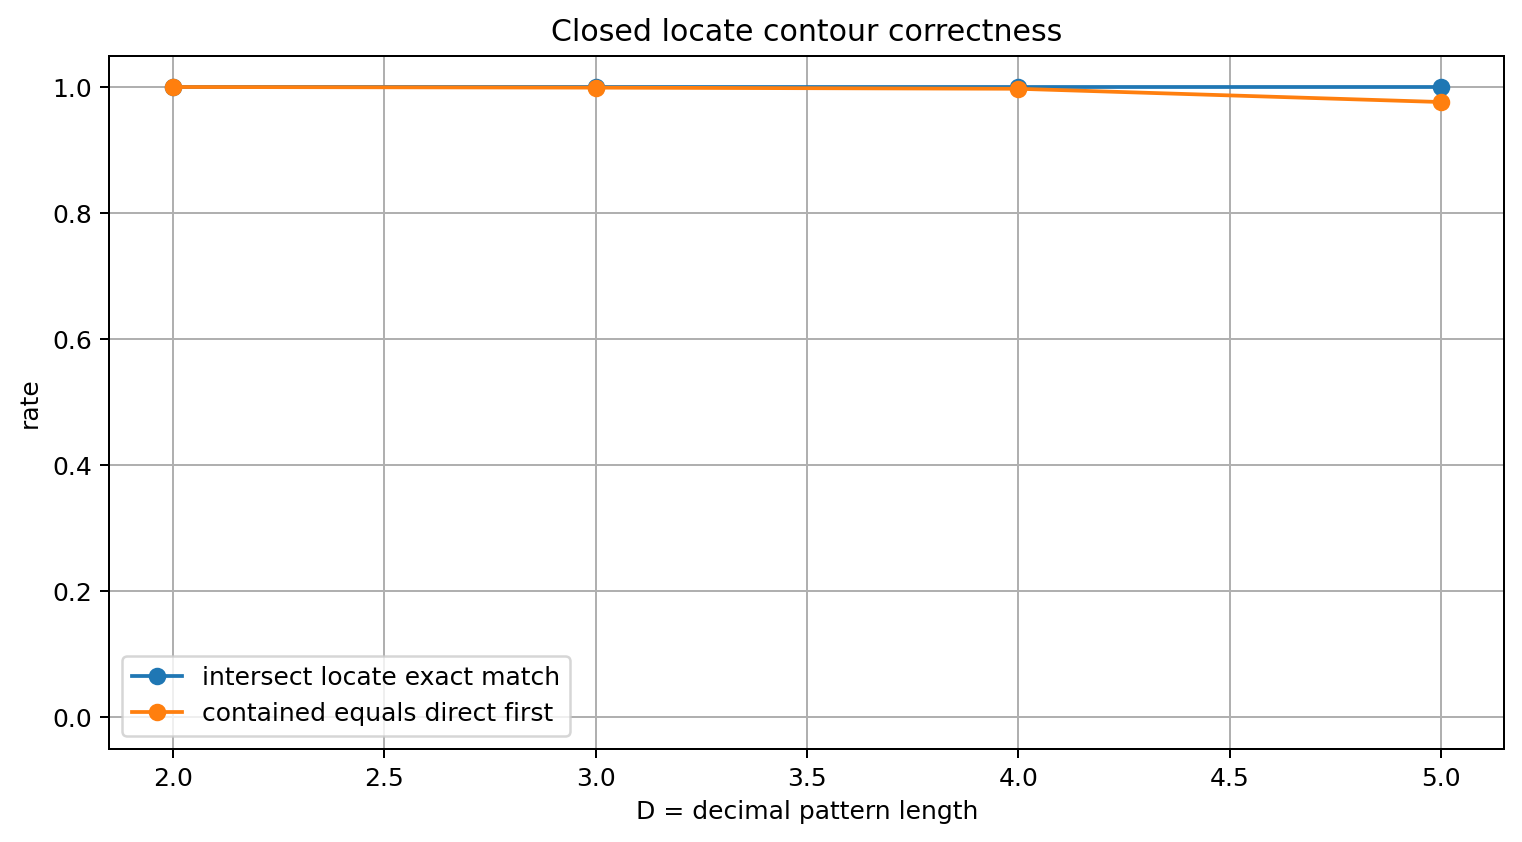
\includegraphics[width=0.82\linewidth]{exp010_correctness.png}
\caption{Experiment 010: совпадение finite locate с direct search.}
\end{figure}

\begin{figure}[H]
\centering
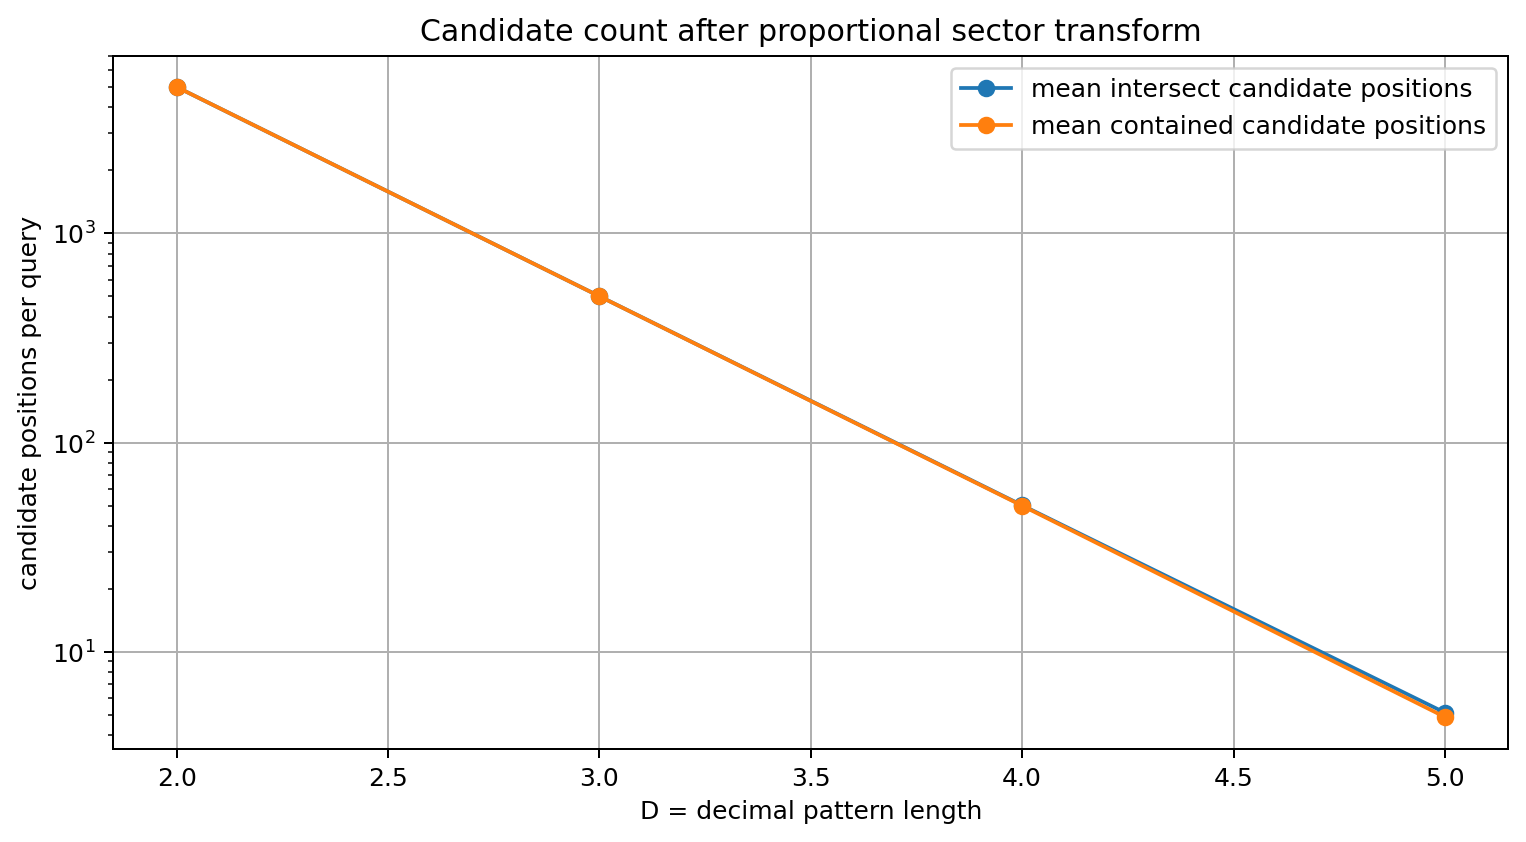
\includegraphics[width=0.82\linewidth]{exp010_candidates.png}
\caption{Experiment 010: число кандидатов после пропорционального перевода уменьшается геометрически с длиной паттерна.}
\end{figure}

\subsection{Обратное дерево и необходимость внешнего сертификата}

Experiment 008 показал, что прямое обращение сектора $[0,10^{-D})$ под действием $f(u)=\{10u\}$ даёт гребёнку из $10^M$ интервалов.  Это объясняет, почему один сертификат попадания не превращается автоматически в формулу первого индекса.

\begin{figure}[H]
\centering
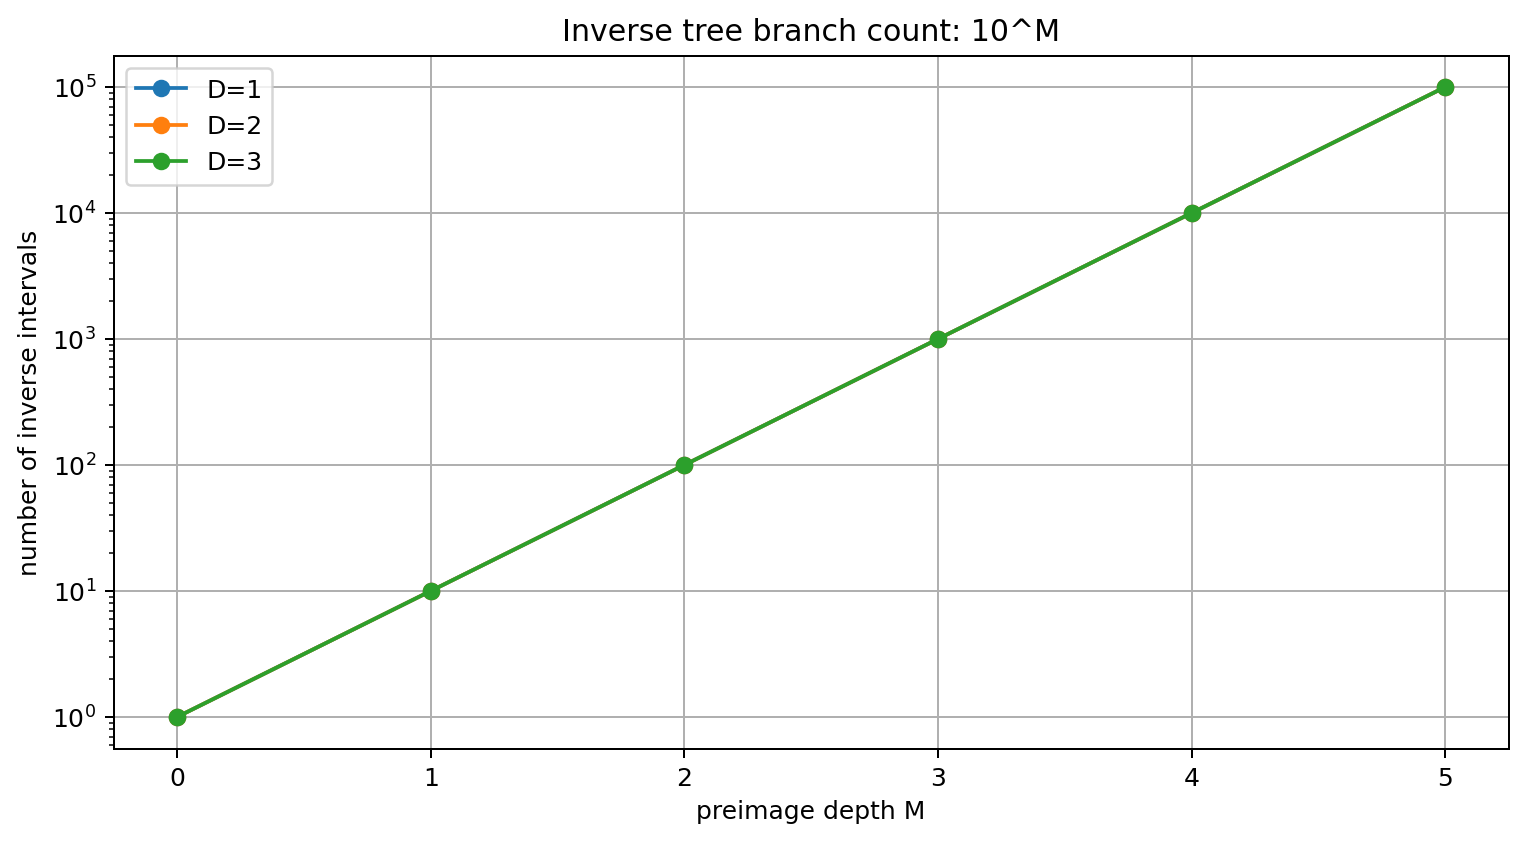
\includegraphics[width=0.78\linewidth]{exp008_inverse_tree.png}
\caption{Experiment 008: количество ветвей обратного дерева растёт как $10^M$.}
\end{figure}

\subsection{Извлечение суффикса из внешнего сектора}

Experiments 014--016 подтвердили лемму внешнего сертификата.  Если другой сектор достаточно узок, то множество кандидатов схлопывается до одного.

\begin{figure}[H]
\centering
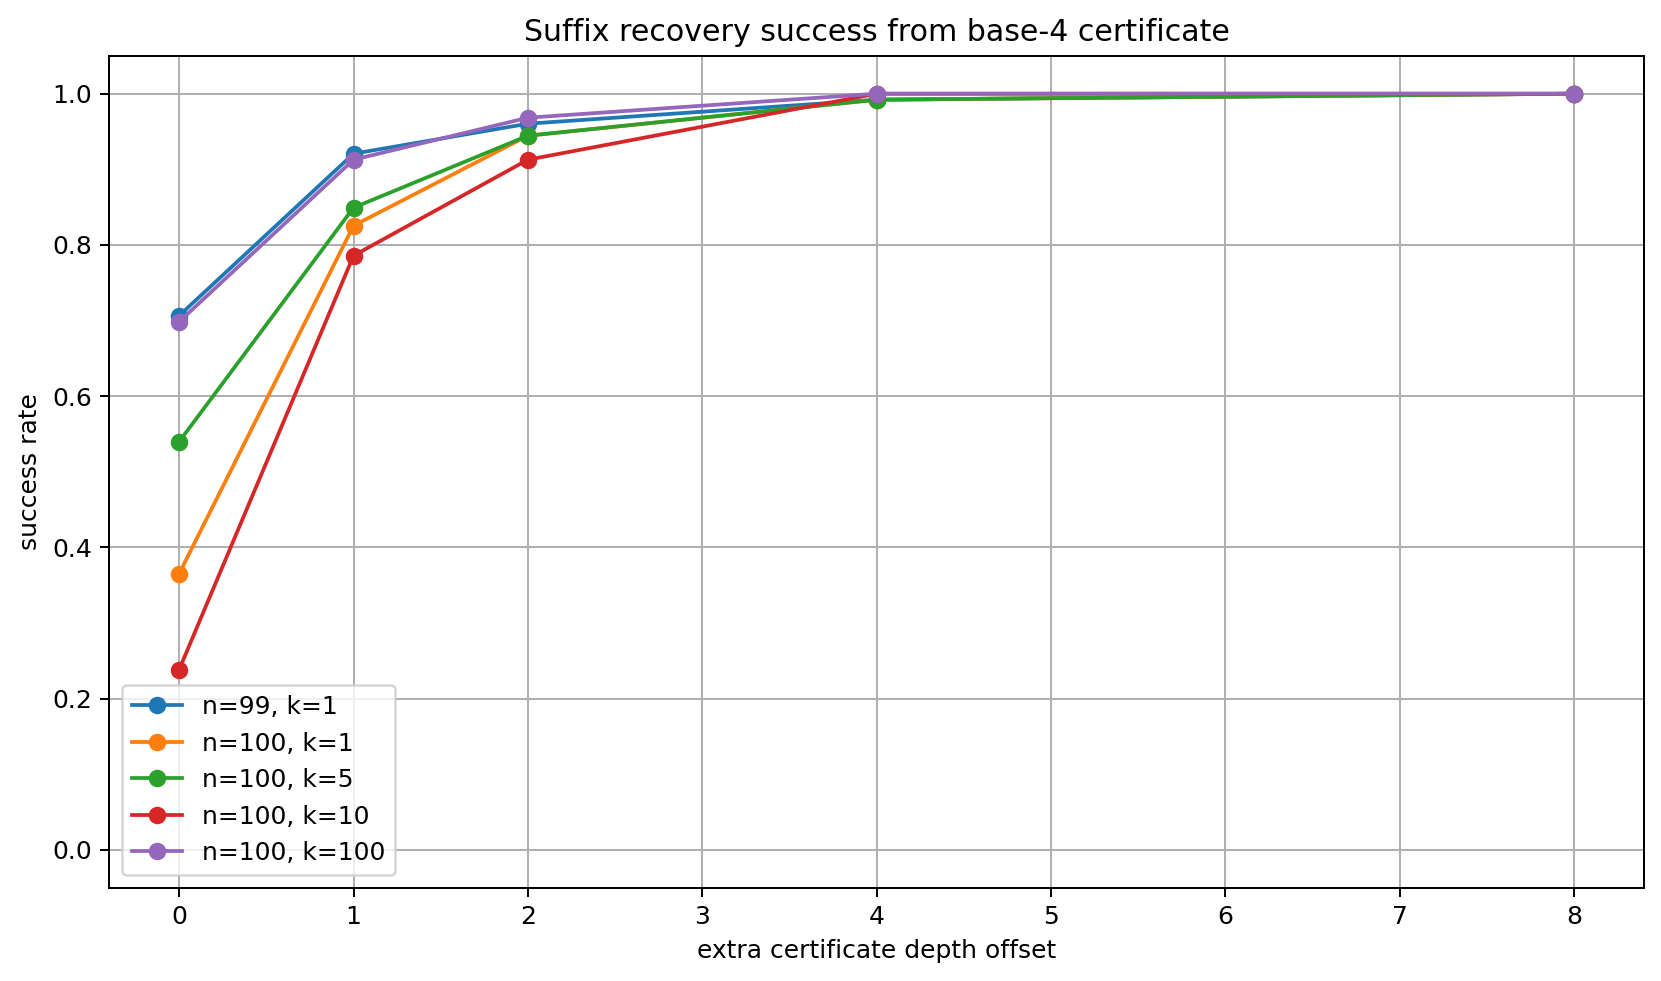
\includegraphics[width=0.78\linewidth]{exp014_success.png}
\caption{Experiment 014: восстановление суффикса из base-4 сертификата при увеличении глубины внешнего сектора.}
\end{figure}

\begin{figure}[H]
\centering
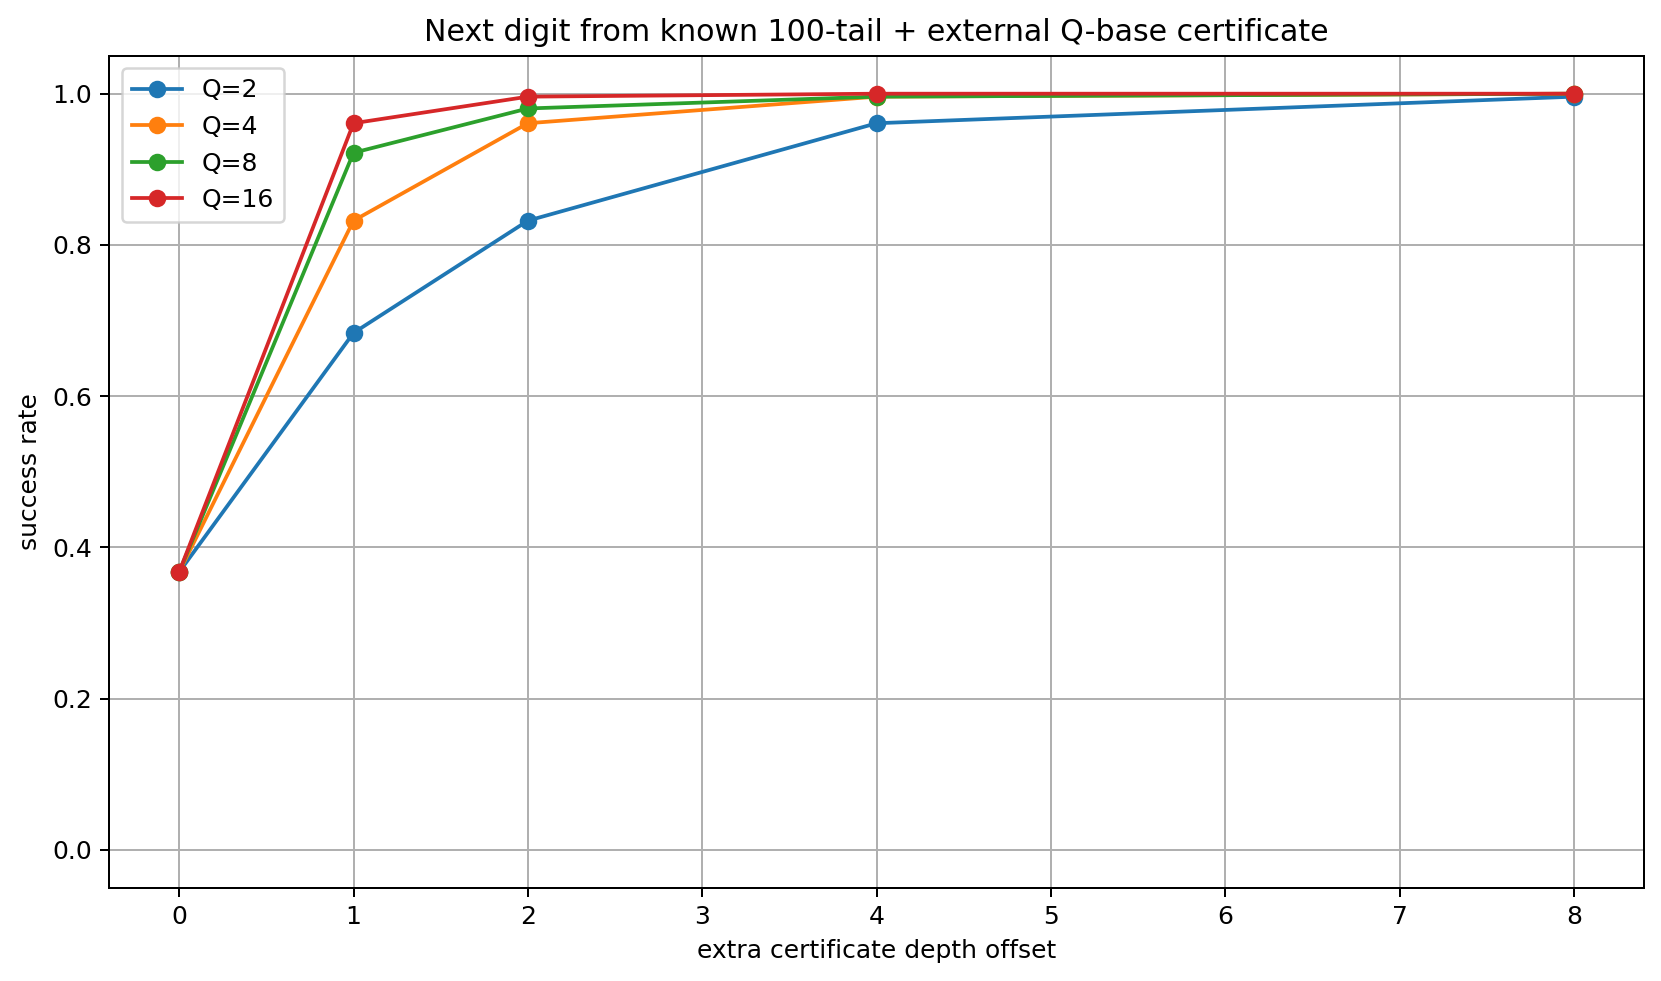
\includegraphics[width=0.78\linewidth]{exp016_next_digit.png}
\caption{Experiment 016: следующая цифра извлекается из внешнего сертификата в базе $Q$.}
\end{figure}

\subsection{Продолжение за искусственной границей}

Experiment 017 восстановил следующие $10$ цифр после искусственной границы $H=2\cdot10^6$:
\[
  \boxed{6121731251}.
\]
Experiment 018 повторил идею с внешним сертификатом из формулы Мэчина
\[
  \pi=16\arctan\frac15-4\arctan\frac1{239},
\]
то есть сертификат не извлекался из скрытого будущего десятичного хвоста.

\begin{figure}[H]
\centering
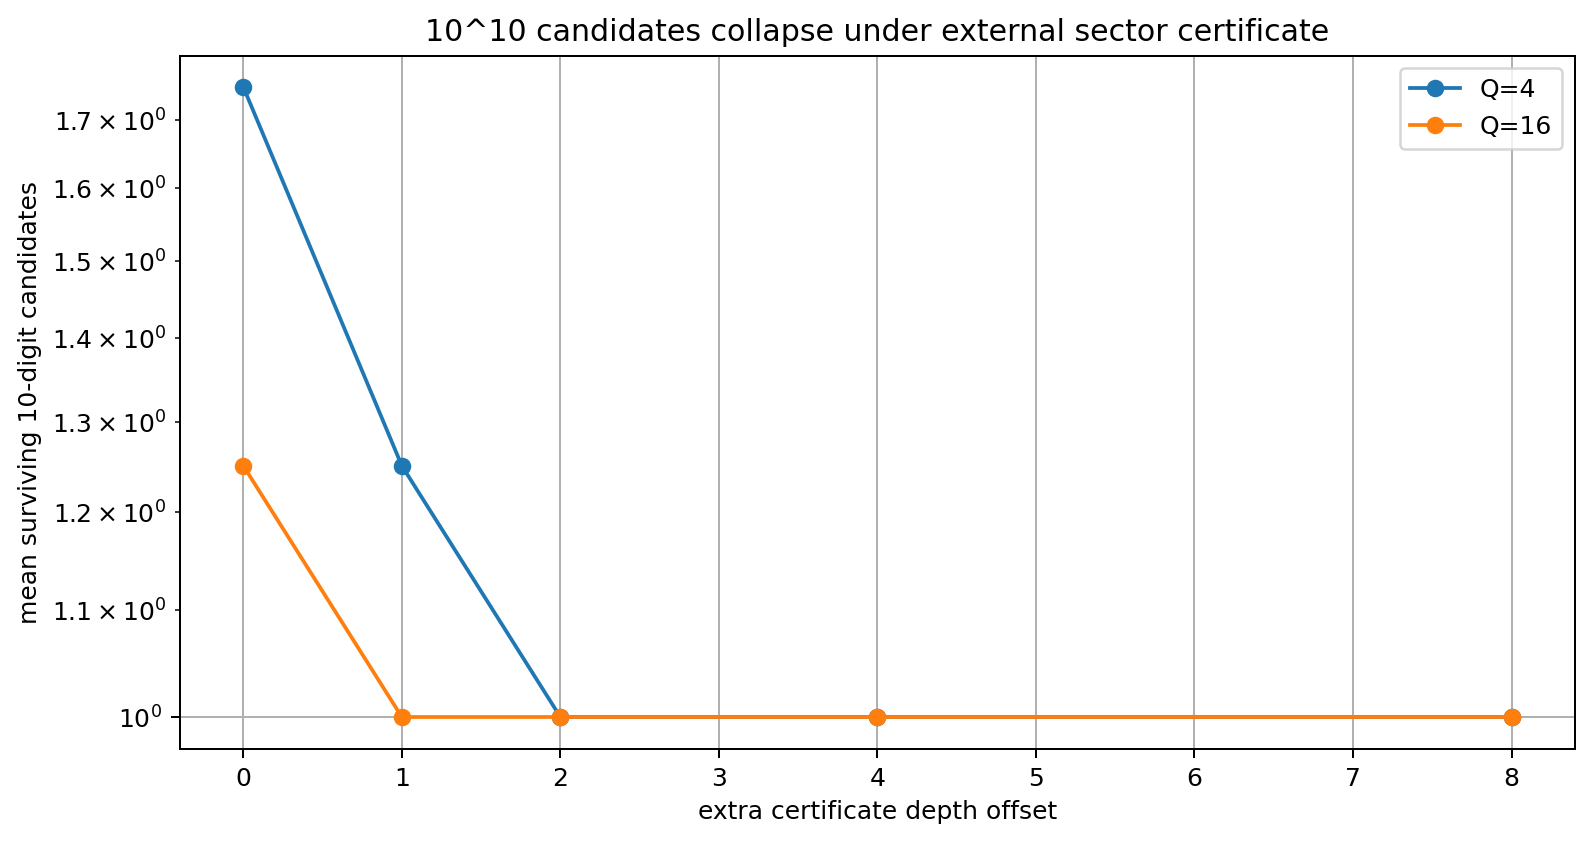
\includegraphics[width=0.78\linewidth]{exp017_next10.png}
\caption{Experiment 017: $10^{10}$ кандидатов десятизначного блока схлопываются под действием внешнего сертификата.}
\end{figure}

\begin{figure}[H]
\centering
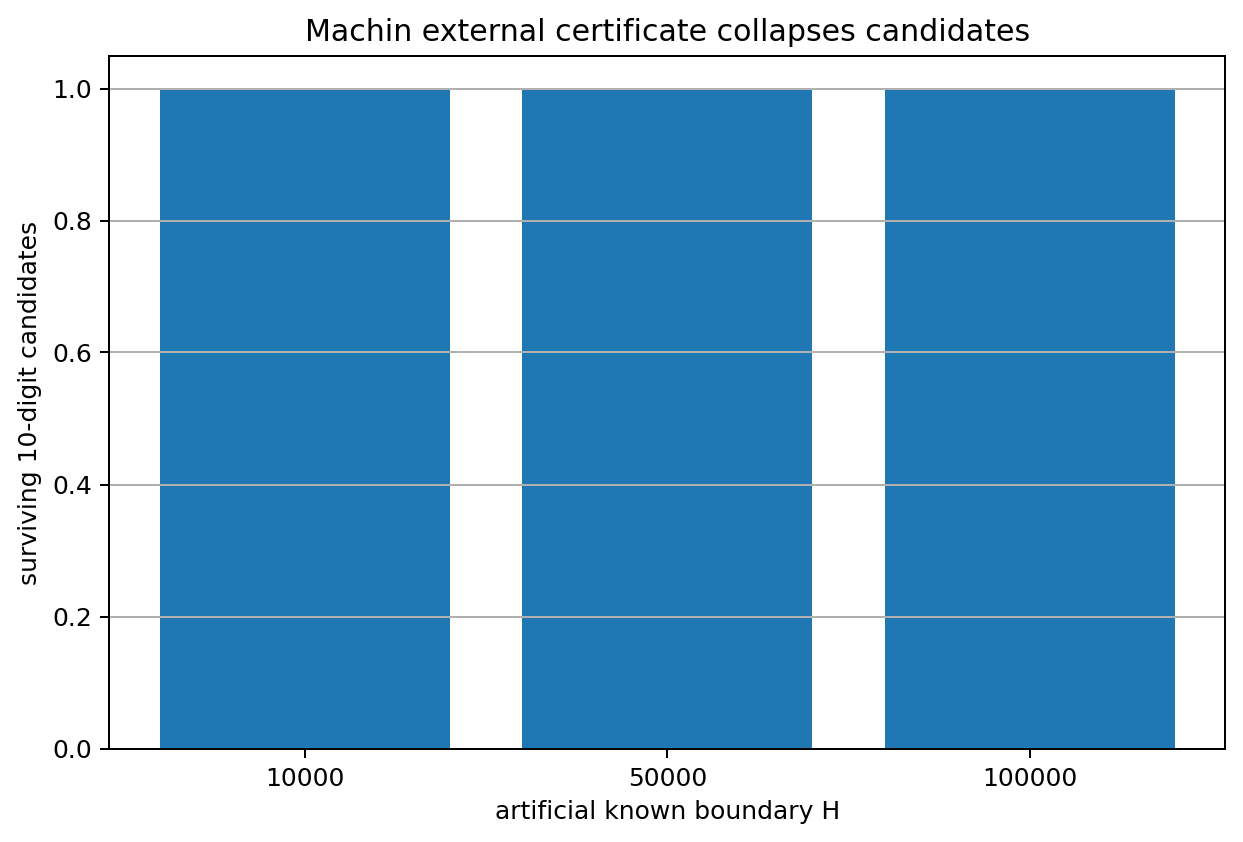
\includegraphics[width=0.78\linewidth]{exp018_machin.png}
\caption{Experiment 018: внешний сертификат из формулы Мэчина оставляет один десятизначный блок на искусственных границах.}
\end{figure}

\section{Что именно теперь можно вычислять}

Пусть известна граница $H$ и последние $N$ цифр перед ней:
\[
  P_N=\operatorname{int}_{10}(\pi[H-N+1:H]).
\]
Пусть нужен следующий блок длины $k$:
\[
  Y\in\{0,\dots,10^k-1\}.
\]
Если существует внешний сертификат для локальной фазы
\[
  \alpha_{H,N}=\fracpart{10^{H-N}\pi},
\]
то есть
\[
  C=\floor{Q^L\alpha_{H,N}},
\]
то следующие $k$ цифр вычисляются как
\[
  Y=A-10^kP_N,
\]
где $A$ - единственное целое число в пересечении
\[
\left[
\floor{\frac{C10^{N+k}}{Q^L}},
\ceil{\frac{(C+1)10^{N+k}}{Q^L}}-1
\right]
\cap
[10^kP_N,10^k(P_N+1)-1].
\]
Если пересечение не одноточечное, требуется более глубокий внешний сертификат.

\section{Обсуждение}

Полученная конструкция не создаёт новую информацию из известного десятичного префикса.  Без внешнего сертификата следующие $k$ цифр имеют $10^k$ кандидатов.  Внешний сертификат является источником уточнения, а пропорциональная арифметика переводит его в десятичную сетку и делает выбор строгим.

Такое разделение важно для честной интерпретации результата:
\begin{itemize}[leftmargin=2em]
  \item известный хвост фиксирует локальный префикс или якорь;
  \item внешний сектор фиксирует более узкое положение фазы;
  \item пропорциональное пересечение извлекает суффикс;
  \item finite index и contained-cells дают сертификаты внутри вычисленного горизонта;
  \item резонансные координаты являются адресным слоем, но пока не доказанным предиктором.
\end{itemize}

Простой suffix/FM-index остаётся базовым конкурентом для поиска строк внутри известного массива цифр.  Отличие фазово-секторной схемы в том, что она возвращает не только позицию, но и proof object: секторное включение или внешний сертификат, который можно проверять арифметически.

\section{Заключение}

Мы построили и проверили фазово-секторную модель адресации цифровых разложений.  Итоговый положительный результат - не предсказатель произвольных будущих цифр $\pi$ из ничего, а замкнутый сертифицирующий контур:
\[
  \text{цель}\to\text{пропорция}\to\text{индекс}\to\text{сертификат}\to\text{адрес},
\]
а также лемма внешнего секторного сертификата, позволяющая алгебраически извлекать следующую цифру или блок цифр при наличии независимого уточнения фазы.  Экспериментальная программа 001--018 показывает путь развития: от резонансных гипотез и отрицательных предикторов к конечному locate-контуру и сертифицированному продолжению через внешние секторы.

\newpage
\begin{thebibliography}{9}
\bibitem{borel1909} E. Borel. Les probabilites denombrables et leurs applications arithmetiques. Rendiconti del Circolo Matematico di Palermo, 1909.
\bibitem{bbp1997} D. H. Bailey, P. B. Borwein, S. Plouffe. On the rapid computation of various polylogarithmic constants. Mathematics of Computation, 1997.
\bibitem{chudnovsky1988} D. V. Chudnovsky, G. V. Chudnovsky. Approximations and complex multiplication according to Ramanujan. In Ramanujan Revisited, 1988.
\bibitem{manbermyers1993} U. Manber, G. Myers. Suffix arrays: a new method for on-line string searches. SIAM Journal on Computing, 1993.
\bibitem{knuth} D. E. Knuth. The Art of Computer Programming, Vol. 2: Seminumerical Algorithms. Addison-Wesley.
\end{thebibliography}

\end{document}
